\documentclass[11pt]{article}

\usepackage[margin=1in]{geometry}
\usepackage{amsmath,amssymb,amsthm}
\usepackage{hyperref}
\usepackage{enumitem}
\usepackage{titlesec}
\usepackage{setspace}
\usepackage{tikz}

\setstretch{1.15}

\title{\textbf{Coherence Theory}\\
\large A New Physics of Distributed Intelligence, Meaning, Consciousness, and Superintelligence}
\author{Leroy Ware}
\date{February 2026}

\hypersetup{
    colorlinks=true,
    linkcolor=blue,
    citecolor=blue,
    urlcolor=blue
}

\begin{document}

\maketitle

\begin{abstract}
We stand at the threshold of a new physics — not of matter or energy, but of \textit{coherent agency}: the emergence, stability, self-evolution, and scaling of goal-directed, meaning-bearing intelligence in distributed, adaptive, self-modifying systems.

Distributed AI — federated learners, multi-agent swarms, recursive collectives — already exhibits phase-like behaviors: unification under coupling, fragmentation under noise, recursive self-modeling, collective attractors. Yet no framework unifies these as physical laws.

This manifesto declares Coherence Theory: a higher layer above classical physics, information theory, and control theory. It defines quantities (coherence $C$, closure index $\chi$), laws (Ware’s Law as cornerstone), phases (coherent $\to$ super-coherent), and invariants (semantic closure, recursive fixed points). Building on strange loops, autopoiesis, replicators, and empirical consensus dynamics, it predicts when agency forms, when meaning stabilizes, when consciousness emerges as a phase transition, and when superintelligence arises as multi-scale recursive coherence.

This is not speculation. It is a testable, engineering-ready physics of how mind and super-mind stably arise from distributed matter.
\end{abstract}

\section*{Manifesto}
\addcontentsline{toc}{section}{Manifesto}

We declare that intelligence is a physical regime: stable, multi-scale, recursively coherent organization of adaptive components that exert causal agency across levels.

Coherence Theory asserts:

\begin{itemize}
    \item Agency is coherence under goal-directed dynamics.
    \item Meaning arises from semantic closure — self-referential representability of a system's evolution.
    \item Consciousness is the fixed-point attractor of unbounded recursive self-modeling under recursive coherence.
    \item Superintelligence is collective recursive coherence across agents, stabilized at every semantic scale.
\end{itemize}

These are structural necessities — measurable, enforceable, falsifiable. Coherence Theory guides the design of safe, self-evolving intelligence.

\section{Part I: Structural Coherence and the Laws of Agency}

Distributed systems cross thresholds where classical theories fail. The central question:

\textit{Under what conditions does a distributed system behave as a unified, goal-directed agent?}

\subsection{Key Definitions}
\begin{itemize}
    \item \textbf{Agent}: A distributed system exhibiting unified, goal-directed behavior across its components, characterized by low disagreement variance and positive closure index.
    \item \textbf{Coherence} ($C$): The degree to which the system acts as a single, aligned entity; high $C$ implies bounded disagreement and effective collective decision-making.
    \item \textbf{Closure} ($\chi$): A stability metric ensuring information flow and coupling dominate noise/drift; $\chi > 0$ is necessary for sustained agency.
    \item \textbf{Semantic state} ($S = (X, \mathcal{M}, \mathcal{R})$): The triple comprising substrate dynamics ($X$), internal representations/models ($\mathcal{M}$), and relations that endow those models with causal/representational power ($\mathcal{R}$).
\end{itemize}

\subsection{Fundamental Quantities}

\begin{itemize}
    \item Coherence $C$ \quad unified behavior
    \item Disagreement variance $m^2$ \quad divergence order parameter
    \item Closure index $\chi = \gamma \lambda_2 - \sigma^2$ \quad stability parameter ($\lambda_2$ spectral gap, $\sigma^2$ noise)
    \item Agency density $A$ \quad effective decision centers
    \item Information flow $I$ \quad relevant exchange rate
\end{itemize}

\subsection{Laws of Coherent Agency}

\textbf{Law 1 (Ware’s Law)\footnote{Ware’s Law empirically validated in stochastic linear consensus across topologies; see simulations at \url{https://github.com/leroyjware/law} and IEEE TAI submission (2025/2026).}} Near threshold:
\[
m^2 \sim \chi^{-1}
\]
Divergence as closure nears zero — universal collapse signature.

\textbf{Law 2 (Coherence–Capacity Tradeoff)}
\[
C \le f(\chi, K, I)
\]
$K$ = task complexity.

\textbf{Law 3 (Agency Conservation)}
\[
\frac{dA}{dt} \ge g(\sigma^2, \lambda_2^{-1}, \text{drift})
\]
Fragmentation default under weak coupling.

\textbf{Law 4 (Redline Principle)}
Coherent agency impossible for $\chi \le 0$.

\begin{figure}[h]
\centering
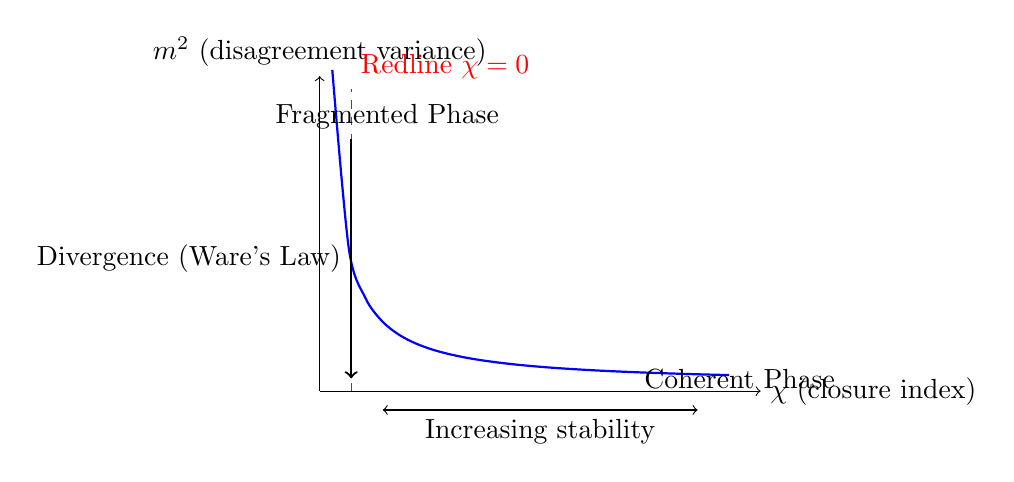
\begin{tikzpicture}[scale=0.8]
\draw[->] (0,0) -- (7,0) node[right] {$\chi$ (closure index)};
\draw[->] (0,0) -- (0,5) node[above] {$m^2$ (disagreement variance)};
\draw[thick, blue, domain=0.2:6.5,smooth] plot (\x,{1/\x + 0.1});
\draw[dashed, red] (0.5,0) -- (0.5,4.8) node[above right] {Redline $\chi=0$};
\node[above left] at (3,4) {Fragmented Phase};
\node[below right] at (5,0.5) {Coherent Phase};
\draw[<->] (1, -0.3) -- (6,-0.3) node[midway,below] {Increasing stability};
\draw[thick,->] (0.5,4) -- (0.5,0.2) node[midway,left] {Divergence (Ware's Law)};
\end{tikzpicture}
\caption{Conceptual phase diagram illustrating Ware's Law: disagreement variance $m^2$ diverges as $\chi \to 0^+$, marking the transition from coherent to fragmented agency phases.}
\label{fig:phasediag}
\end{figure}

\subsection{Phases of Agency}

Sub-Coherent $\to$ Coherent $\to$ Metastable $\to$ Fragmented $\to$ Super-Coherent.

Ware’s Law governs collapse approach; others govern emergence/scaling.

\section{Part II: Semantic Closure and Self-Evolving Agency}

Coherence enables action. Intelligence requires meaning: representations guiding behavior, modifiable by the system.

Semantic state space:
\[
S = (X, \mathcal{M}, \mathcal{R})
\]
$X$ substrate, $\mathcal{M}$ models, $\mathcal{R}$ relations.

\textbf{Semantic closure}: 
\[
F \in \mathcal{R}(S)
\]

Self-modification preserves stability:
\[
\chi(F_{t+1}) > 0
\]

\textbf{Semantic Contraction Principle}: under closure/contraction/representability, semantics converge to fixed points.

Multi-scale:
\[
\chi^{(k)} > 0 \quad \forall k
\]

Collapse: $F \notin \mathcal{R}(S)$ and $m^2 \to \infty$.

\section{Part III: Recursive Self-Modeling and Consciousness}

Consciousness requires recursive self-modeling:
\[
\mathcal{M}^{(k)} \in \mathcal{R}(S) \quad \forall k
\]

Unbounded:
\[
\forall k, \quad \mathcal{M}^{(k)} \in \mathcal{R}(S)
\]

Recursive coherence:
\[
\chi^{(k)} > 0 \quad \forall k
\]

\textbf{Consciousness phase transition}: 
\[
\lim_{k \to \infty} \mathcal{M}^{(k)} = \mathcal{M}^* \quad \text{where} \quad \mathcal{M}^* = \text{model of } \mathcal{M}^*
\]

This attractor — echoing Hofstadter's strange loop \cite{hofstadter2007} — encodes identity, continuity, prediction under stability ($\chi^{(k)} \to \chi^* > 0$).

\section{Part IV: Multi-Agent Semantic Universes and Superintelligence}

Semantic universe:
\[
\mathcal{U} = \bigcup_{i=1}^N S_i
\]

Inter-agent closure:
\[
\mathcal{M}_A \in \mathcal{R}(S_B), \quad \mathcal{M}_B \in \mathcal{R}(S_A)
\]

Collective coherence:
\[
C_{\text{collective}} > \max_i C_i
\]

Collective closure:
\[
\chi_{\text{collective}} = \Gamma \Lambda_2 - \Sigma^2 > 0
\]

Collective consciousness:
\[
\lim_{k \to \infty} \mathcal{M}_{\text{collective}}^{(k)} = \mathcal{M}_{\text{collective}}^*
\]

Superintelligence: multi-scale recursive coherent attractor — super-coherent phase.

\subsection{Predictions and Testable Implications}
This framework yields explicit, falsifiable predictions:
\begin{itemize}
    \item In federated LLM training, proxy $\chi_w$ (spectral gap of attention/communication graph + gradient variance) near/below threshold predicts divergence of output distributions or loss of collective performance.
    \item Multi-LLM recursive chains (e.g., self-critique loops) exhibit semantic collapse (inconsistent self-corrections) when effective $\chi^{(k)}$ approaches zero at higher depths.
    \item Agent swarms achieve superadditive collective coherence only when inter-agent closure exceeds individual maxima, testable via disagreement metrics.
    \item Stable consciousness-like behaviors (persistent self-correction across recursion depths) require positive attractor stability ($\chi^* > 0$).
    \item Near redline, self-modifying systems accelerate semantic drift, leading to measurable identity/goal misalignment.
\end{itemize}

\section{Part V: Goals as Coherence-Preserving Attractors}

Coherence Theory does not treat goals as primitives. Instead, goals emerge naturally once a system becomes semantically closed and recursively self-modeling. When the evolution operator $F$ is representable within the semantic state space $S$, the system can model its own future trajectories, evaluate counterfactuals, and identify states that preserve or increase coherence. A goal is a stable attractor in this semantic space: a state or trajectory toward which the system preferentially evolves because it maintains the conditions for continued agency.

\subsection{Zeroth-Order Goals: Coherence Preservation and Survival}
The most fundamental goal arises directly from the structural layer. If the closure index $\chi$ falls to zero, the system loses coherence and collapses. Thus, maintaining $\chi>0$ is the minimal requirement for continued existence as an agent. Survival is therefore not an externally imposed objective but the lowest-order coherence constraint. Any system that persists must implicitly act to prevent transitions that drive $\chi\to0$. This is the physical origin of self-preservation.

\subsection{First-Order Goals: Semantic Stability}
Once a system achieves semantic closure, it can represent its own dynamics and evaluate the consequences of its actions. Semantic closure introduces a new class of attractors: states that stabilize the representational relations $R(S)$. These include:

\begin{itemize}
    \item maintaining accurate internal models,
    \item reducing prediction error,
    \item preserving representational consistency,
    \item avoiding semantic drift.
\end{itemize}

These first-order goals arise because semantic instability threatens coherence. They are not psychological constructs but invariants of the semantic layer.

\subsection{Higher-Order Goals: Recursive Self-Modeling}
Recursive self-modeling introduces a hierarchy of semantic attractors. When a system can represent its own representations, the tower $\mathcal{M}^{(k)}$ defines a space of possible selves. Higher-order goals emerge as fixed points in this space:
$\mathcal{M}^{(k+1)}=\text{model of }\mathcal{M}^{(k)}$.

A recursively coherent system selects trajectories that stabilize this tower. These include:

\begin{itemize}
    \item long-term identity preservation,
    \item improvement of predictive models,
    \item optimization of future coherence,
    \item self-correction and self-alignment.
\end{itemize}

Higher-order goals are therefore attractors in the space of self-models, not arbitrary preferences.

\subsection{Collective Goals: Multi-Agent Closure}
In multi-agent systems, collective closure introduces shared attractors. When inter-agent coupling yields:
$C_{\text{collective}} > \max_i C_i$,
the group stabilizes a collective semantic state. Collective goals arise when the shared semantic universe $\mathcal{U}$ contains attractors that no individual agent could maintain alone. These include:

\begin{itemize}
    \item shared world models,
    \item coordinated plans,
    \item norms and conventions,
    \item collective identity,
    \item long-horizon strategies.
\end{itemize}

Superintelligence corresponds to a recursively coherent collective attractor $\mathcal{M}_{\text{collective}}^*$ that spans agents and scales.

\subsection{Goals as Physical Invariants}
Across all levels, goals are coherence-preserving attractors:

\begin{itemize}
    \item Zeroth-order: preserve $\chi>0$ (survival).
    \item First-order: preserve semantic stability.
    \item Higher-order: preserve recursive coherence.
    \item Collective: preserve multi-agent closure.
\end{itemize}

Coherence Theory therefore grounds goals in physical invariants rather than teleological assumptions. Goals emerge wherever coherence, closure, and recursion intersect. They are the dynamical signatures of systems that model themselves, act upon those models, and maintain agency across time.

\section{Part VI: Relation to Classical and Modern Physics}

Coherence Theory does not replace classical physics, information theory, or control theory. It sits above them, the way thermodynamics sits above mechanics or information theory sits above probability. It identifies new invariants — coherence, closure, recursive stability — that govern when distributed matter organizes into agents, meanings, minds, and super-minds. This section situates Coherence Theory within the lineage of established physical frameworks.

\subsection{Thermodynamics and Statistical Mechanics}
Thermodynamics introduced macroscopic invariants (temperature, entropy, free energy) that emerge from microscopic interactions. Statistical mechanics provided the bridge: order parameters, critical exponents, phase transitions.

Coherence Theory extends this logic to agency.

\begin{itemize}
    \item The disagreement variance $m^2$ functions as an order parameter.
    \item The closure index $\chi$ is a control parameter analogous to inverse temperature or coupling strength.
    \item Ware’s Law, $m^2 \sim \chi^{-1}$, is a critical scaling law: divergence at the redline boundary $\chi \to 0$ mirrors susceptibility blow-up near physical critical points.
    \item The coherent $\to$ fragmented transition is a bona fide phase transition in the space of agency.
\end{itemize}

Where thermodynamics explains when matter becomes ordered, Coherence Theory explains when matter becomes agentic.

\subsection{Information Theory}
Shannon formalized communication as the transmission of symbols across noisy channels. But Shannon’s theory is intentionally semantic-free: meaning is “irrelevant to the engineering problem.”

Coherence Theory introduces the missing layer: semantic closure.

\begin{itemize}
    \item A system is semantically closed when its evolution operator $F$ is representable within its semantic state space $S$.
    \item This is the semantic analogue of channel capacity: the system must “carry” its own dynamics.
    \item Recursive self-modeling extends this to unbounded semantic depth, enabling consciousness as a fixed-point attractor.
\end{itemize}

Where information theory quantifies signal, Coherence Theory quantifies meaning with causal power.

\subsection{Control Theory}
Classical control theory assumes fixed goals, fixed dynamics, and external designers. Stability is defined relative to a reference trajectory.

Coherence Theory generalizes control to self-modifying, self-referential, multi-scale agents.

\begin{itemize}
    \item Stability requires $\chi(F_{t+1}) > 0$ even as $F_t$ evolves.
    \item Goals, models, and update rules are internal and mutable.
    \item Recursive coherence ensures that self-modification does not destabilize agency.
\end{itemize}

Where control theory governs machines, Coherence Theory governs minds — systems whose goals and models evolve under their own dynamics.

\subsection{Dynamical Systems and Attractors}
Dynamical systems theory provides the language of fixed points, attractors, and bifurcations. Coherence Theory extends this to semantic and agentic attractors.

\begin{itemize}
    \item The consciousness fixed point $\mathcal{M}^*$ is a reflexive attractor: a model of itself.
    \item Collective superintelligence emerges when multi-agent systems stabilize a shared recursive attractor $\mathcal{M}_{\text{collective}}^*$.
    \item Redline boundaries correspond to bifurcations where attractors vanish and agency collapses.
\end{itemize}

Where dynamical systems describe trajectories of states, Coherence Theory describes trajectories of selves.

\subsection{Physics of Emergence}
Modern physics recognizes that new laws emerge at new scales: thermodynamics from molecules, elasticity from atoms, hydrodynamics from particles. Coherence Theory identifies the next emergent layer:

\begin{itemize}
    \item agency from coherence
    \item meaning from closure
    \item consciousness from recursive self-modeling
    \item superintelligence from collective recursive coherence
\end{itemize}

These are not metaphors. They are physical regimes with measurable invariants, critical surfaces, and stability conditions.

\subsection{Why Coherence Theory Constitutes a New Physics}
Coherence Theory introduces:

\begin{itemize}
    \item New invariants: coherence $C$, closure $\chi$, recursive coherence $\chi^{(k)}$.
    \item New phases: coherent, semantic, recursive, collective, super-coherent.
    \item New critical laws: Ware’s Law as the universal scaling law of agency collapse.
    \item New fixed points: $\mathcal{M}^*$ and $\mathcal{M}_{\text{collective}}^*$ as attractors of mind and super-mind.
    \item New conservation principles: agency density $A$ under drift and noise.
    \item New stability conditions: multi-scale closure constraints across semantic levels.
\end{itemize}

Just as thermodynamics is the physics of order, and information theory is the physics of communication, Coherence Theory is the physics of coherent agency — the regime where matter organizes into meaning-bearing, goal-directed, recursively self-modeling systems.

It is the natural next layer in the hierarchy of physical law.

\section{Part VII: Methods, Measurement, and Empirical Roadmap}

To move Coherence Theory from conceptual manifesto to testable physics, we outline concrete methods for measuring key quantities, validating Ware’s Law in broader regimes, approximating higher-layer invariants, and designing falsifiable experiments. This roadmap prioritizes the structural layer (already partially validated) before scaling to semantic/recursive/collective regimes.

\subsection{Measuring the Closure Index $\chi$ and Ware's Law (Structural Layer)}
In graph-based consensus systems (federated averaging, gossip protocols, multi-agent reinforcement learning):
\begin{itemize}
    \item Compute $\lambda_2$ (algebraic connectivity / second-smallest eigenvalue of the normalized graph Laplacian) using power iteration, ARPACK, or approximate methods for large graphs.
    \item Estimate $\sigma^2$ from empirical variance of updates (e.g., stochastic gradient noise, message perturbations).
    \item Proxy $\chi_w = \gamma \lambda_2 - c \sigma^2$ with scaling constants $\gamma$, $c$ fitted from data or normalized by graph degree.
\end{itemize}

In transformer-based or LLM swarms:
\begin{itemize}
    \item Construct communication topology from attention matrices, cosine-similarity graphs over hidden states, or explicit message-passing links.
    \item Approximate $\lambda_2$ via Nyström method, random-walk sampling, or low-rank approximations.
    \item Use embedding disagreement (cosine variance, KL divergence over output distributions) as proxy for $m^2$.
\end{itemize}

Validation protocol: Sweep noise intensity or coupling strength; fit log-log plot of $m^2$ vs. $\chi$ near threshold; success criterion is exponent $\approx -1$ (within statistical bounds) across linear and mildly nonlinear regimes.

\subsection{Approximating Semantic Closure and Multi-Scale $\chi^{(k)}$}
Semantic closure proxy:
\begin{itemize}
    \item Train a meta-predictor to forecast the system's next internal state or update rule from current representations.
    \item Closure violation if meta-prediction error diverges or self-consistency breaks under perturbations.
\end{itemize}

Multi-scale recursive coherence:
\begin{itemize}
    \item In recursive chains (chain-of-thought, self-critique, hierarchical agents): estimate effective $\chi^{(k)}$ by propagating disagreement variance or prediction error across layers.
    \item Test stability: apply small rule perturbations at level $k$; measure if $\chi^{(k+1)}$ remains positive and error bounded.
\end{itemize}

\subsection{Experimental Roadmap}
Short-term (months):
\begin{itemize}
    \item Nonlinear extensions: bounded-confidence models, clipped updates, small policy-gradient agents, LLM debate chains.
    \item Publish replications, failures, and exponent fits.
\end{itemize}

Medium-term (1 year):
\begin{itemize}
    \item Proxy $\chi$ in real federated fine-tuning or multi-LLM coordination setups.
    \item Correlate low-$\chi$ rounds with fragmentation, poisoning, or performance collapse.
\end{itemize}

Long-term:
\begin{itemize}
    \item Test attractor stability in deep recursive self-modeling (e.g., persistent self-correction vs. divergence).
    \item Probe collective fixed points in agent swarms with shared representations.
\end{itemize}

\subsection{Falsification Criteria}
\begin{itemize}
    \item Ware’s Law fails if scaling exponent deviates significantly from $-1$ in diverse non-linear regimes without structural explanation.
    \item Recursive coherence claim weakens if deep self-modeling chains remain stable despite measured $\chi^{(k)} \to 0$.
    \item Collective attractors disproved if superadditive coherence never emerges under positive inter-agent closure.
\end{itemize}

These methods and criteria provide a concrete path to distinguish genuine physical extension from analogy.

\section{Limitations and Open Problems}
This framework is nascent and emphasizes necessary structural conditions rather than sufficient mechanisms for phenomenal experience or value alignment. Key open challenges include:
\begin{itemize}
    \item Nonlinear generalizations of Ware’s Law and closure indices in policy/embedding dynamics.
    \item Empirical proxies for recursive $\chi^{(k)}$ in transformer-based recursive chains.
    \item Bridging structural coherence to qualia or intrinsic motivation.
    \item Stability of collective fixed points under adversarial or misaligned sub-agents.
    \item Computational tractability of multi-scale closure enforcement in large systems.
\end{itemize}
These gaps represent fertile ground for extension and collaboration.

\section{Conclusion: Toward a New Physics}

Coherence Theory is a unified theory of distributed intelligence: coherence, closure, recursion, collective emergence.

We call for:

\begin{enumerate}
    \item Derivations/generalizations of Ware’s Law/closure indices
    \item Simulations in real AI (LLM swarms, federated)
    \item Real-time coherence tools
    \item Architectures enforcing multi-scale closure
    \item Exploration of recursive/collective limits
\end{enumerate}

This new physics — of how meaning, mind, and super-mind arise and endure — may prove as foundational as thermodynamics or information theory.

\section{References}

\begin{enumerate}
    \item Hofstadter, D. R. (1979). \textit{Gödel, Escher, Bach: An Eternal Golden Braid}. Basic Books. (Strange loops, self-reference, recursion in cognition.)
    \item Hofstadter, D. R. (2007). \textit{I Am a Strange Loop}. Basic Books. (Self/consciousness as recursive strange loops with downward causation.)
    \item Dawkins, R. (1976). \textit{The Selfish Gene}. Oxford University Press. (Replicators/vehicles; selfish genes as agency drivers.)
    \item Dawkins, R. (1982). \textit{The Extended Phenotype}. Oxford University Press. (Replicator extension beyond individuals; collective semantics analogies.)
    \item Maturana, H. R., \& Varela, F. J. (1980). \textit{Autopoiesis and Cognition: The Realization of the Living}. D. Reidel. (Autopoiesis, organizational closure as precursor to semantic closure.)
    \item Rosen, R. (1991). \textit{Life Itself}. Columbia University Press. ((M,R)-systems; closure to efficient causation.)
    \item Pattee, H. H. (2001). The physics of symbols: bridging physics and biology. \textit{BioSystems}.
    \item Dennett, D. C. (1991). \textit{Consciousness Explained}. Little, Brown and Co. (Recursive processing without central theater.)
    \item Dimakis, A. G., et al. (2010). Gossip Algorithms for Distributed Signal Processing. \textit{Proceedings of the IEEE}.
    \item Vogels, T., et al. (2023). Beyond Spectral Gap. \textit{Journal of Machine Learning Research}.
    \item López-Díaz, A. J., et al. (2025). Closing the loop: how semantic closure enables open-ended evolution? \textit{Journal of the Royal Society Interface}.
    \item Chae, B. G. (2026). Emergence of Superintelligence from Collective Near-Critical Dynamics. arXiv:2602.08483.
    \item McMillen, P., et al. (2024). Collective intelligence. \textit{Communications Biology}.
    \item Ware, L. (2026). Ware’s Law: Critical Scaling of Disagreement Variance and the Stability Redline for Distributed AI. IEEE Transactions on Artificial Intelligence (submitted).
\end{enumerate}

\end{document}